\chapter{A ferramenta desenvolvida}

Para o desenvolvimento do software livraria Dom Casmurro foi utilizado as seguintes ferramentas:


\section{Linguagem de programação}
 A linguagem de programação utilizada foi a linguem Java, muito utilizada em desenvolvimento para desktop e web. É uma linguagem orientada a objetos,fortemente tipada e multiplataforma, de modo que uma vez compilado o código, é possivel executa-lo em qualquer sistema que disponha de uma maquina virtual Java;

\section{Ambiente de desenvolvimento}
 O ambiente utilizado para o desenvolvimento do código do programa foi o software NetBeans IDE versão 8.0.1; focada no desenvolvimento utilizando a linguagem de programação Java.

\section{Persistência de dados}
 O armazenamento das informações como por exemplo os cadastro das operações de cliente, funcionários, fornecedores e livros são inseridos no banco de dados Mysql Server 5.6;

O software utilizado para o desenvolvimento do banco de dados foi o MySQL Workbench 6.0 CE. Tem como função a modelagem e gerenciamento dos dados, onde gera as tabelas e seus relacionamentos, podendo inserir dados nessas tabelas e efetuar a sincronização entre modelo lógico e a base de dados física.


\section{Requisitos Funcionais}

\begin{itemize}

\item Ao abrir o software a tela de login é exibida, mostrando os campos “usuário” e “senha”, com dois botões, um “acessar” o software, e outro para “cancelar” a operação;

\item Se o botão “Cancelar” for pressionado é exibida uma mensagem de aviso: “Tem certeza que deseja encerrar a operação?” se “sim” a mensagem de aviso some e o programa é automaticamente fechado; se “não” a mensagem é fechada e permanece na tela de login;

\item Se o botão “Acessar” for pressionado o software verifica se a senha está correta: “empresa123”, a tela principal do software é exibida. E a tela de login é fechada. Caso a “senha” esteja incorreta o software exibe uma mensagem de aviso: “Senha incorreta” e limpa os campo para que possa ser novamente preenchido.

\item Na tela principal do software é exibido um menu com as seguintes informações “Cadastrar”, “Consultar”, “Editar”, “Deletar” e “sobre”;

\item Se qualquer uma das opções do menu for pressionado: será exibido um submenu: “Cliente”, “Funcionário”, “Fornecedor”, “Livros”;

\item No “cadastro” o usuário poderá cadastrar os “Cliente”, “Funcionário”, “Fornecedor”, “Livros”, na base de dados;

\item Na “Consulta” o usuário poderá ter acesso as informações armazenada na base de dados, de qualquer uma das opções mencionadas acima;

\item Em “Editar” o usuário poderá acrescentar, remover ou alterar informações dos cadastros feitos;

\item Caso seja necessário o menu com a opção “Deletar” fará com que o usuário possa remover os  cadastros realizados até o então.

\item Se  “Sobre” do menu principal for selecionado será exibido uma tela com as informações do software e quem o desenvolveu;


\end{itemize}


\section{Requisitos Não Funcionais}

\begin{itemize}

\item O software é deve ser desenvolvido na linguagem de programação Java, aproveitando sua natureza mutiplataforma e pela mesma fazer parte da ementa do curso Técnico em Informática;

\item Para executar nosso programa com sobra de recursos é necessário uma máquina com um processador Intel Atom de 1,7 GHZ com 2GB de memória RAM;

\item É executado em qualquer plataforma seja ela Linux, Windows;
\end{itemize}

\section {UML do software (Diagrama de USE CASE)}

A construção da UML no desenvolvimento do software trouxe vários benefícios, pois nos auxiliou na modelagem e 
documentação do sistema. Nele foi construído as definições de cada uma das operações. A figura \ref{uml_cliente}
representa o Diagrama de Casos de Uso do Cliente. A seguir tem-se a descrição de cada uma das açoes possíveis para
o cliente.

%=================================================================================

\begin{figure}[ht]
	\centering 
	\caption{UML Cliente}
	
	\label{uml_cliente}
	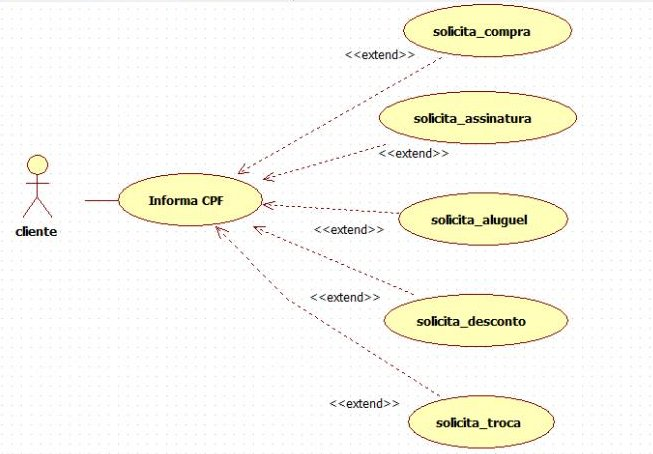
\includegraphics[scale = 0.7]{imagens/uml-cliente.jpg}
	\\Fonte: Do autor
\end{figure}


\begin{itemize}
\item Cliente informa seu CPF para o funcionários
\item Cliente solicitar uma compra de livros;
\item Cliente solicita assinatura mensal de livros;
\item Cliente solicita o aluguel dos livros;
\item Cliente solicita desconto na compra de um livro;
\item Cliente solicita a troca dos livros;
\end{itemize}

A figura \ref{uml_funcionario} representa o Diagrama de Casos de Uso do
Funcionário. A seguir tem-se a descrição de cada uma das açoes possíveis para
o usuário.

%=================================================================================
%UML FUNCIONARIO 

\begin{figure}[ht]
	\centering 
	\caption{UML Funcionario}
	\label{uml_funcionario}
	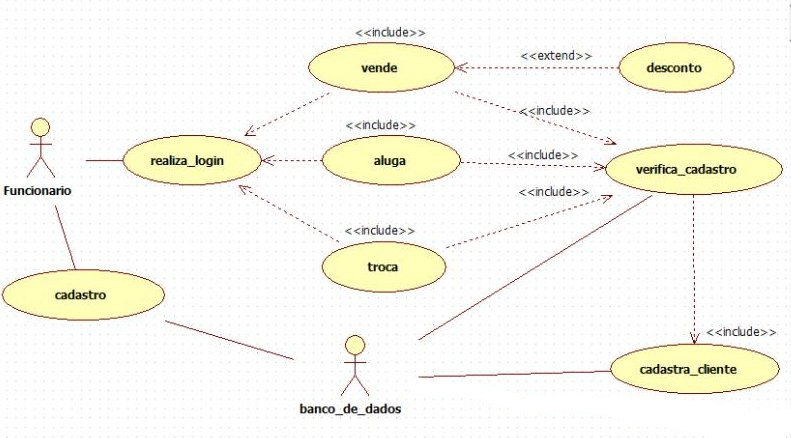
\includegraphics[scale = 0.50]{imagens/uml-funcionario.jpg}
	\\Fonte: Do autor
\end{figure}

\begin{itemize}
\item Funcionário realiza cadastro e armazena no banco de dados;
\item Funcionário realiza login no sistema;
\item Funcionário vende, troca, aluga livros para o cliente;
\item Funcionário oferece desconto na venda do livro;
\item Funcionário verifica o cadastro na venda, troca e aluguel dos livros;
\item Se cliente não for cadastrado: Funcionário cadastra Cliente no Banco de dados;
\end{itemize}

%=================================================================================
A figura \ref{uml_fornecedor} representa o Diagrama de Casos de Uso do
Fornecedor. A seguir tem-se a descrição de cada uma das açoes possíveis para
o fornecedor.

\begin{itemize}
\item Fornecedor informa CPF para o funcionário;
\item Se Fornecedor não cadastrado funcionário o cadastra no banco de dados;
\item Fornecedor vende livro para a empresa;
\item Fornecedor solicita desconto na venda dos livros;os;
\end{itemize}

\begin{figure}[h]
	\centering 
	\caption{UML Fornecedor}
	\label{uml_fornecedor}
	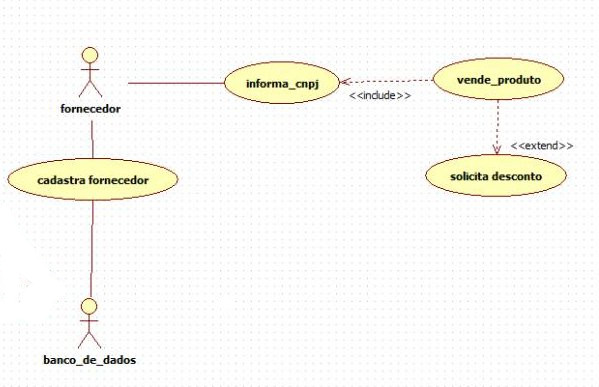
\includegraphics[scale = 0.70]{imagens/uml-fornecedor.jpg}
	\\Fonte: Do autor
\end{figure}





%=================================================================================
\newpage
\section{Fluxograma}

O fluxograma é uma representação gráfica de um processo ou rotina de trabalho geralmente feito através de figuras geométricas e retas que demonstram, de forma descomplicada, a transição de informações entre os elementos que o compõem.

Pode ser definido também como o gráfico em que se representa o curso ou caminho percorrido por certo elemento;

O fluxograma é fundamental para simplificação e racionalização do trabalho, permitindo um estudo detalhado dos métodos, processos e rotinas de um departamento ou área da organização. 


\begin{figure}[H]
	\centering 
	\caption{Floxograma}
	
	\label{loxograma}
	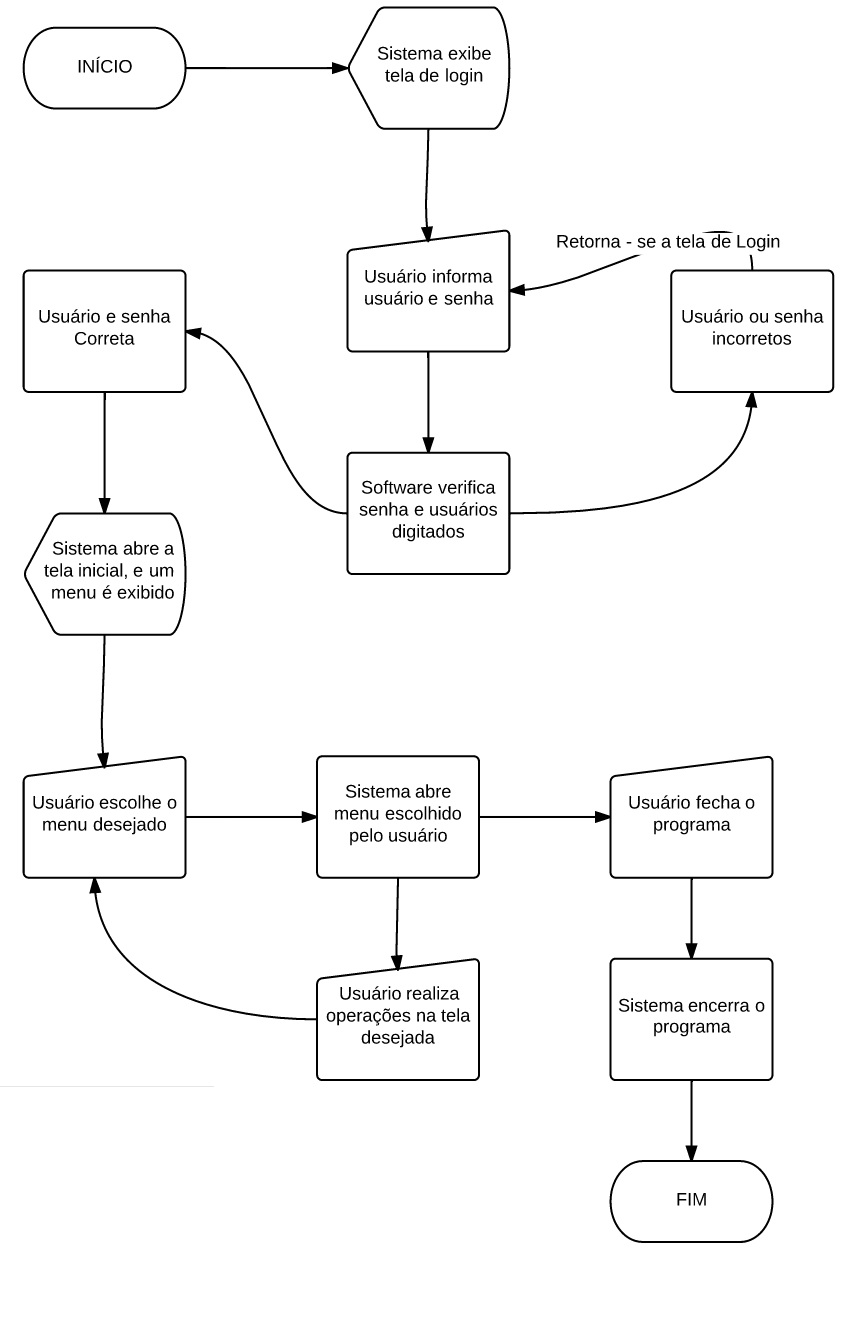
\includegraphics[scale = 0.70]{imagens/fluxo.jpg}
	\\Fonte: Do autor
\end{figure}

\newpage

%==================================================================================
\section{Contrução do banco de dados}
\subsection{Tabela cliente}
